\documentclass[12pt,a4paper,oneside]{book}

\usepackage[utf8]{inputenc}
\usepackage[T1]{fontenc}
\usepackage{lmodern}
\usepackage{graphicx}
\usepackage{amsmath,amssymb}
\usepackage{geometry}
\usepackage{hyperref}
\usepackage{xcolor}
\usepackage{listings}
\usepackage{microtype}
\usepackage{booktabs}
\usepackage{caption}
\usepackage{placeins}
\usepackage{tikz}
\usetikzlibrary{arrows.meta, positioning, fit, backgrounds, calc, shapes.geometric}

\geometry{margin=1in}
\emergencystretch=1.5em

% Float tuning to preserve strict chronological document order and prevent orphan gaps
\renewcommand{\topfraction}{0.90}
\renewcommand{\bottomfraction}{0.85}
\renewcommand{\textfraction}{0.10}
\renewcommand{\floatpagefraction}{0.80}

\makeatletter
\newcommand{\chapterauthor}[1]{%
  {\parindent0pt\vspace*{-15pt}%
  \linespread{1.1}\large\itshape\begin{flushright}#1\end{flushright}%
  \par\nobreak\vspace*{25pt}}
  \@afterheading%
}
\makeatother

% =====================================================================
% Syntax Highlighting Configuration for C++
% =====================================================================
\definecolor{codeblue}{rgb}{0.0, 0.2, 0.75}
\definecolor{codegreen}{rgb}{0.13, 0.55, 0.13}
\definecolor{codegray}{rgb}{0.42, 0.42, 0.42}
\definecolor{codepurple}{rgb}{0.55, 0.0, 0.75}
\definecolor{backcolour}{rgb}{0.97, 0.98, 0.99}
\definecolor{indigo}{RGB}{75, 0, 130}

% Architecture Diagram Color Palette
\definecolor{layer1bg}{HTML}{F8F9FA}
\definecolor{layer1border}{HTML}{6C757D}
\definecolor{uiboxbg}{HTML}{EFF6FF}

\definecolor{layer2bg}{HTML}{F1F5F9}
\definecolor{layer2border}{HTML}{3B82F6}

\definecolor{layer3bg}{HTML}{F0FDF4}
\definecolor{layer3border}{HTML}{16A34A}
\definecolor{writerbg}{HTML}{DCFCE7}
\definecolor{filebg}{HTML}{BBF7D0}
\definecolor{fileborder}{HTML}{166534}
\definecolor{filetext}{HTML}{14532D}

\definecolor{darkborder}{HTML}{1E293B}
\definecolor{subtitlegray}{HTML}{4B5563}
\definecolor{dividergray}{HTML}{CBD5E1}
\definecolor{badgeborder}{HTML}{94A3B8}

\lstdefinestyle{cppstyle}{
    backgroundcolor=\color{backcolour},   
    commentstyle=\color{codegreen}\itshape,
    keywordstyle=\color{codeblue}\bfseries,
    numberstyle=\tiny\color{codegray},
    stringstyle=\color{codepurple},
    basicstyle=\ttfamily\footnotesize,
    breakatwhitespace=false,         
    breaklines=true,                 
    captionpos=b,                    
    keepspaces=true,                 
    numbers=left,                    
    numbersep=6pt,                  
    showspaces=false,                
    showstringspaces=false,
    showtabs=false,                  
    tabsize=2,
    frame=lines,
    rulecolor=\color{black!25}
}
\lstset{style=cppstyle}

\hypersetup{
    colorlinks=true,
    linkcolor=blue!70!black,
    citecolor=blue!70!black,
    urlcolor=blue!70!black
}

\begin{document}

\mainmatter

% =====================================================================
% C++ OOP Mini-Project Chapter Submission
% Group Number: 24 (Section numbering starts with 24.1, 24.2, ...)
% File: 24_Audio_Synthesizer.tex
% =====================================================================

\setcounter{chapter}{23}

\chapter[Audio Synthesizer (WAV Generator)]{Audio Synthesizer (WAV Generator): Algorithmic Sound Synthesis and RIFF/WAVE Binary Serialization}
\chaptermark{Audio Synthesizer (WAV Generator)}
\markboth{CHAPTER 24. AUDIO SYNTHESIZER (WAV GENERATOR)}{CHAPTER 24. AUDIO SYNTHESIZER (WAV GENERATOR)}
\chapterauthor{Shailesh (251150), Sirthik (251153)}

% =====================================================================
% 24.1 INTRODUCTION AND PROBLEM STATEMENT
% =====================================================================
\section{Introduction and Problem Statement}
Sound synthesis represents the mathematical intersection of physics, digital signal processing (DSP), and computer systems engineering. In an era where audio generation is often abstracted away behind monolithic third-party multimedia frameworks (such as SDL, PortAudio, or OpenAL), understanding the low-level generation of acoustic pressure waves from mathematical primitives provides fundamental insights into memory efficiency, real-time algorithms, and low-level binary data serialization.

The primary objective of this project is to architect and implement an extensible, decoupled, and highly performant \textbf{Audio Synthesizer and WAV Generator} in modern C++ (C++17). The system is engineered from the ground up without relying on external multimedia runtimes for audio generation or file formatting. Instead, the application directly generates discrete periodic waveforms, modulates their amplitude across temporal domains using an Attack-Decay-Sustain-Release (ADSR) envelope generator, and formats the synthesized raw pulse-code modulation (PCM) audio samples into a standard Microsoft Resource Interchange File Format (RIFF) WAVE audio file via unbuffered binary C++ file streams (\texttt{std::ofstream}).

The engineering requirements stipulated for the project comprise:
\begin{enumerate}
    \item \textbf{Waveform Generation:} Mathematically generate three fundamental periodic acoustic waveforms: pure sinusoidal waves (\textit{Sine}), odd-harmonic rich pulses (\textit{Square}), and full harmonic-spectrum ramps (\textit{Sawtooth}).
    \item \textbf{Object-Oriented Architecture:} Implement an abstract base class \texttt{Oscillator} defining a pure virtual polymorphic interface for dynamic sample generation, alongside dedicated derived classes implementing concrete mathematical transfer functions.
    \item \textbf{Temporal Dynamic Envelope:} Implement an encapsulated \texttt{Envelope} class providing four-stage piecewise linear ADSR modulation to prevent acoustic clicking artifacts caused by instantaneous step transients.
    \item \textbf{Raw Binary Serialization:} Assemble canonical 44-byte RIFF/WAVE file headers and serialize 16-bit signed integer little-endian audio samples into persistent storage using formatted binary C++ file streams (\texttt{std::ofstream}).
    \item \textbf{Defensive Validation:} Guard against acoustic aliasing by strictly enforcing the Nyquist-Shannon sampling theorem limit ($0 < f < f_s / 2$) and clamping peak amplitude values to prevent integer overflow.
    \item \textbf{Dual Frontend Interaction:} Deliver both a scriptable Command-Line Interface (CLI) supporting parameterized flags and an interactive Terminal User Interface (TUI) powered by FTXUI featuring real-time oscilloscopic waveform previews.
\end{enumerate}

From an end-user perspective, the system provides sound designers, audio researchers, and students with an intuitive utility capable of generating calibrated acoustic test signals, musical tones, and customized synthesis sweeps exported directly into high-fidelity uncompressed 16-bit PCM \texttt{.wav} files compatible with any industry-standard media player or digital audio workstation (DAW).

% =====================================================================
% 24.2 SCOPE AND FEATURE SET
% =====================================================================
\section{Scope and Feature Set}
The project delivers an end-to-end audio rendering pipeline partitioned into a static synthesis library (\texttt{synth\_core}) and frontend driver executables. The feature set includes:

\begin{itemize}
    \item \textbf{Feature 1 (Multi-Waveform Timbre Generation):} Algorithmic synthesis of three fundamental wave profiles:
    \begin{itemize}
        \item \textit{Sine Wave:} Pure fundamental frequency ($f$) devoid of harmonic overtones ($x(n) = \sin(2\pi \phi_n)$).
        \item \textit{Square Wave:} Composed exclusively of odd integer harmonics ($f, 3f, 5f, \dots$) decaying at $1/n$ amplitude ($x(n) = \text{sgn}(\sin(2\pi \phi_n))$).
        \item \textit{Sawtooth Wave:} Composed of both even and odd harmonics decaying at $1/n$ ($x(n) = 2\phi_n - 1$).
    \end{itemize}

    \item \textbf{Feature 2 (Continuous Normalized Phase Accumulation):} A normalized phase accumulator $\phi \in [0.0, 1.0)$ updated as $\phi_{n+1} = (\phi_n + f / f_s) \pmod{1.0}$, maintaining sample-accurate phase tracking across arbitrary sampling frequencies ($f_s$).

    \item \textbf{Feature 3 (Piecewise Linear ADSR Dynamic Envelope):} A 4-stage time-domain amplitude modulator:
    \begin{itemize}
        \item \textit{Attack ($T_A$):} Linear ramp from zero amplitude to maximum gain ($1.0$).
        \item \textit{Decay ($T_D$):} Linear ramp down from peak amplitude to configured sustain level.
        \item \textit{Sustain ($S$):} Maintained steady-state amplitude plateau ($S \in [0.0, 1.0]$).
        \item \textit{Release ($T_R$):} Linear decay from sustain down to silence ($0.0$).
    \end{itemize}

    \item \textbf{Feature 4 (Direct RIFF/WAVE Binary Stream Serialization):} Direct byte-level Little-Endian bit encoding and memory packing for the standard 44-byte canonical WAV header without relying on compiler-dependent struct packing.

    \item \textbf{Feature 5 (Defensive Boundary Validation and Nyquist Safety):} Enforces $0 < f < f_s / 2$, clamps amplitude values to $[-1.0, 1.0]$ to prevent clipping, and validates non-negative envelope timing parameters.

    \item \textbf{Feature 6 (Dual Presentation Frontends):}
    \begin{itemize}
        \item \textit{CLI Executable (\texttt{synth}):} Optimized for rapid shell scripting and automated testing via standard flags.
        \item \textit{Interactive TUI (\texttt{synth-tui}):} Interactive terminal dashboard built using FTXUI featuring real-time Braille-canvas oscilloscopic previews.
    \end{itemize}
\end{itemize}

% ---------------------------------------------------------------------
% 24.2.1 TECHNOLOGY STACK
% ---------------------------------------------------------------------
\subsection{Technology Stack}
Table~\ref{tab:tech_stack} provides a comprehensive overview of the technologies, tools, and libraries utilized across the engineering lifecycle.

\begin{table}[htbp]
\centering
\caption{Comprehensive Technology Stack of the Audio-WAV-Synthesizer Project}
\label{tab:tech_stack}
\footnotesize
\setlength{\tabcolsep}{5pt}
\begin{tabular}{@{}p{2.4cm}p{2.6cm}p{2.1cm}p{1.6cm}p{6.5cm}@{}}
\toprule
\textbf{Layer / Domain} & \textbf{Technology} & \textbf{Standard} & \textbf{License} & \textbf{Architectural Rationale} \\ \midrule
\textbf{Primary Language} & Modern C++ & ISO/IEC C++17 & Open ISO & Deterministic memory management (RAII), zero-overhead abstractions, compile-time type safety. \\
\textbf{DSP Core} & C++ Standard Library & C++17 STL & ISO & Contiguous sample buffers and fixed-width integer types without external third-party runtimes. \\
\textbf{Binary File I/O} & \texttt{std::ofstream} & C++ Stream & ISO & Unbuffered raw binary file output with manual little-endian byte serialization. \\
\textbf{Build System} & CMake & Version 3.14+ & BSD 3-Cl. & Declarative target-based orchestration; partitions engine into static library and dual executables. \\
\textbf{TUI Interface} & FTXUI & Version 5.0.0 & MIT & Declarative functional terminal UI providing interactive parameter sliders and keyboard controls. \\
\textbf{Waveform Preview} & \texttt{ftxui::Canvas} & FTXUI Comp. & MIT & Visualizer rendering continuous waveforms using Unicode Braille dot matrices. \\
\textbf{Audio Format} & Microsoft RIFF/WAVE & Canonical 1991 & Open Spec & Uncompressed 16-bit linear PCM audio container with universal DAW and player support. \\
\textbf{Verification} & Audacity \& Hex Dumps & v3.x / CLI & GPL v2 / OS & FFT spectrum analysis, envelope inspection, and hexadecimal verification of WAV headers. \\
\bottomrule
\end{tabular}
\end{table}

\FloatBarrier

% =====================================================================
% 24.3 OBJECT-ORIENTED ARCHITECTURE
% =====================================================================
\section{Object-Oriented Architecture}
The software architecture adheres rigorously to established Object-Oriented Programming (OOP) principles, guaranteeing high cohesion, loose coupling, and strict separation of concerns across audio synthesis, data modulation, and binary persistence.

\begin{enumerate}
    \item \textbf{Data Abstraction:} 
    The abstract base class \texttt{Oscillator} establishes a formal contract for periodic acoustic signal generators. Callers interact exclusively with the pure virtual member function \texttt{nextSample()}, abstracting away underlying trigonometric evaluations, phase increments, and piecewise boundary calculations (Listing~\ref{lst:oscillator_h}).

\begin{lstlisting}[language=C++, caption={Abstract Oscillator Base Class (\texttt{include/Oscillator.h})}, label={lst:oscillator_h}]
#pragma once

class Oscillator {
public:
    Oscillator(double frequency, double sampleRate);
    virtual ~Oscillator() = default;

    virtual double nextSample() = 0; // Pure virtual polymorphic interface

    void setFrequency(double frequency);
    void reset();

protected:
    void advancePhase();

    double frequency_;
    double sampleRate_;
    double phase_ = 0.0; // Normalized phase tracking [0.0, 1.0)
};
\end{lstlisting}

    \item \textbf{Polymorphism and Dynamic Dispatch:} 
    The core synthesis pipeline in \texttt{render()} operates uniformly on an abstract base pointer \texttt{std::unique\_ptr<Oscillator>}. Dynamic dispatch resolves invocations of \texttt{nextSample()} to the appropriate concrete waveform realization selected via a Factory Method pattern (Listing~\ref{lst:synth_cpp}).

\begin{lstlisting}[language=C++, caption={Polymorphic Factory and Rendering Pipeline (\texttt{src/Synth.cpp})}, label={lst:synth_cpp}]
#include "SynthSettings.h"
#include "Envelope.h"
#include "Waveforms.h"
#include <memory>
#include <vector>

static std::unique_ptr<Oscillator> makeOscillator(const SynthSettings& s) {
    switch (s.waveform) {
        case Waveform::Square:
            return std::make_unique<SquareOscillator>(s.frequency, s.sampleRate);
        case Waveform::Sawtooth:
            return std::make_unique<SawtoothOscillator>(s.frequency, s.sampleRate);
        case Waveform::Sine:
        default:
            return std::make_unique<SineOscillator>(s.frequency, s.sampleRate);
    }
}

std::vector<double> render(const SynthSettings& s) {
    const std::size_t total = static_cast<std::size_t>(s.duration * s.sampleRate);
    std::unique_ptr<Oscillator> osc = makeOscillator(s);
    Envelope env(s.attack, s.decay, s.sustain, s.release, s.sampleRate);

    std::vector<double> samples;
    samples.reserve(total);

    for (std::size_t i = 0; i < total; ++i) {
        const double wave = osc->nextSample();
        const double gain = env.amplitudeAt(i, total);
        samples.push_back(wave * gain * s.amplitude);
    }
    return samples;
}
\end{lstlisting}

    \item \textbf{Encapsulation and Information Hiding:} 
    Internal state attributes—such as accumulated phase and envelope parameters—are strictly encapsulated with \texttt{private} or \texttt{protected} access specifiers, mutating solely through validated member functions (Listing~\ref{lst:envelope_cpp}).

\begin{lstlisting}[language=C++, caption={Encapsulated ADSR Dynamic Envelope Modulator (\texttt{src/Envelope.cpp})}, label={lst:envelope_cpp}]
#include "Envelope.h"
#include <algorithm>

Envelope::Envelope(double attack, double decay, double sustain, double release,
                   double sampleRate)
    : attack_(attack), decay_(decay), sustain_(sustain), release_(release),
      sampleRate_(sampleRate) {}

double Envelope::amplitudeAt(std::size_t sampleIndex,
                             std::size_t totalSamples) const {
    const double t = static_cast<double>(sampleIndex) / sampleRate_;
    const double length = static_cast<double>(totalSamples) / sampleRate_;

    double gain;
    if (attack_ > 0.0 && t < attack_) {
        gain = t / attack_;
    } else if (decay_ > 0.0 && t < attack_ + decay_) {
        gain = 1.0 - (1.0 - sustain_) * ((t - attack_) / decay_);
    } else {
        gain = sustain_;
    }

    if (release_ > 0.0) {
        gain *= std::clamp((length - t) / release_, 0.0, 1.0);
    }
    return gain;
}
\end{lstlisting}

    \item \textbf{Inheritance and Code Reusability:} 
    The derived oscillator classes publicly inherit from \texttt{Oscillator}, directly reusing the underlying phase accumulator while overriding concrete waveform transfer functions (Listing~\ref{lst:waveforms_cpp}).

\begin{lstlisting}[language=C++, caption={Concrete Derived Waveform Implementations (\texttt{src/Waveforms.cpp})}, label={lst:waveforms_cpp}]
#include "Waveforms.h"
#include <cmath>

namespace {
constexpr double kTwoPi = 6.283185307179586476925286766559;
}

double SineOscillator::nextSample() {
    const double sample = std::sin(kTwoPi * phase_);
    advancePhase();
    return sample;
}

double SquareOscillator::nextSample() {
    const double sample = (phase_ < 0.5) ? 1.0 : -1.0;
    advancePhase();
    return sample;
}

double SawtoothOscillator::nextSample() {
    const double sample = 2.0 * phase_ - 1.0;
    advancePhase();
    return sample;
}
\end{lstlisting}

    \item \textbf{Separation of Concerns (SoC):} 
    The system isolates mathematical sound generation (\texttt{Oscillator}), amplitude modulation (\texttt{Envelope}), configuration parameters (\texttt{SynthSettings}), low-level binary serialization (\texttt{WavWriter}), and presentation frontends into decoupled compilation units.
\end{enumerate}

% =====================================================================
% 24.3.1 CLASS DESIGN AND ASSOCIATIONS
% =====================================================================
\subsection{Class Design and Associations}
The relationships between the primary architectural components are structured as follows:
\begin{itemize}
    \item \textbf{Generalization (Inheritance):} \texttt{SineOscillator}, \texttt{SquareOscillator}, and \texttt{SawtoothOscillator} publicly inherit from the abstract base class \texttt{Oscillator}, realizing the pure virtual interface \texttt{nextSample()}.
    \item \textbf{Composition:} The rendering pipeline (\texttt{render()}) instantiates and manages the lifecycle of an \texttt{Oscillator} (via \texttt{std::unique\_ptr}) and an \texttt{Envelope} instance for the duration of the audio synthesis task.
    \item \textbf{Aggregation / Association:} The \texttt{SynthSettings} Plain Old Data (POD) structure aggregates configuration values alongside the strongly typed enumeration \texttt{Waveform}.
    \item \textbf{Dependency:} The static utility class \texttt{WavWriter} depends upon normalized \texttt{std::vector<double>} sample buffers produced by \texttt{render()} and interacts directly with \texttt{std::ofstream} binary sinks.
\end{itemize}

% =====================================================================
% 24.4 SYSTEM ARCHITECTURE AND UML MODELING
% =====================================================================
\section{System Architecture and UML Modeling}
The system adopts a decoupled three-tier architecture: the \textbf{User Interface Layer}, the \textbf{Core Synthesizer Engine} (\texttt{synth\_core} static library), and the \textbf{Storage and Output Layer}. Figure~\ref{fig:sys_arch} illustrates this high-level architectural decomposition.

\begin{figure}[htbp]
\centering
\resizebox{0.92\textwidth}{!}{%
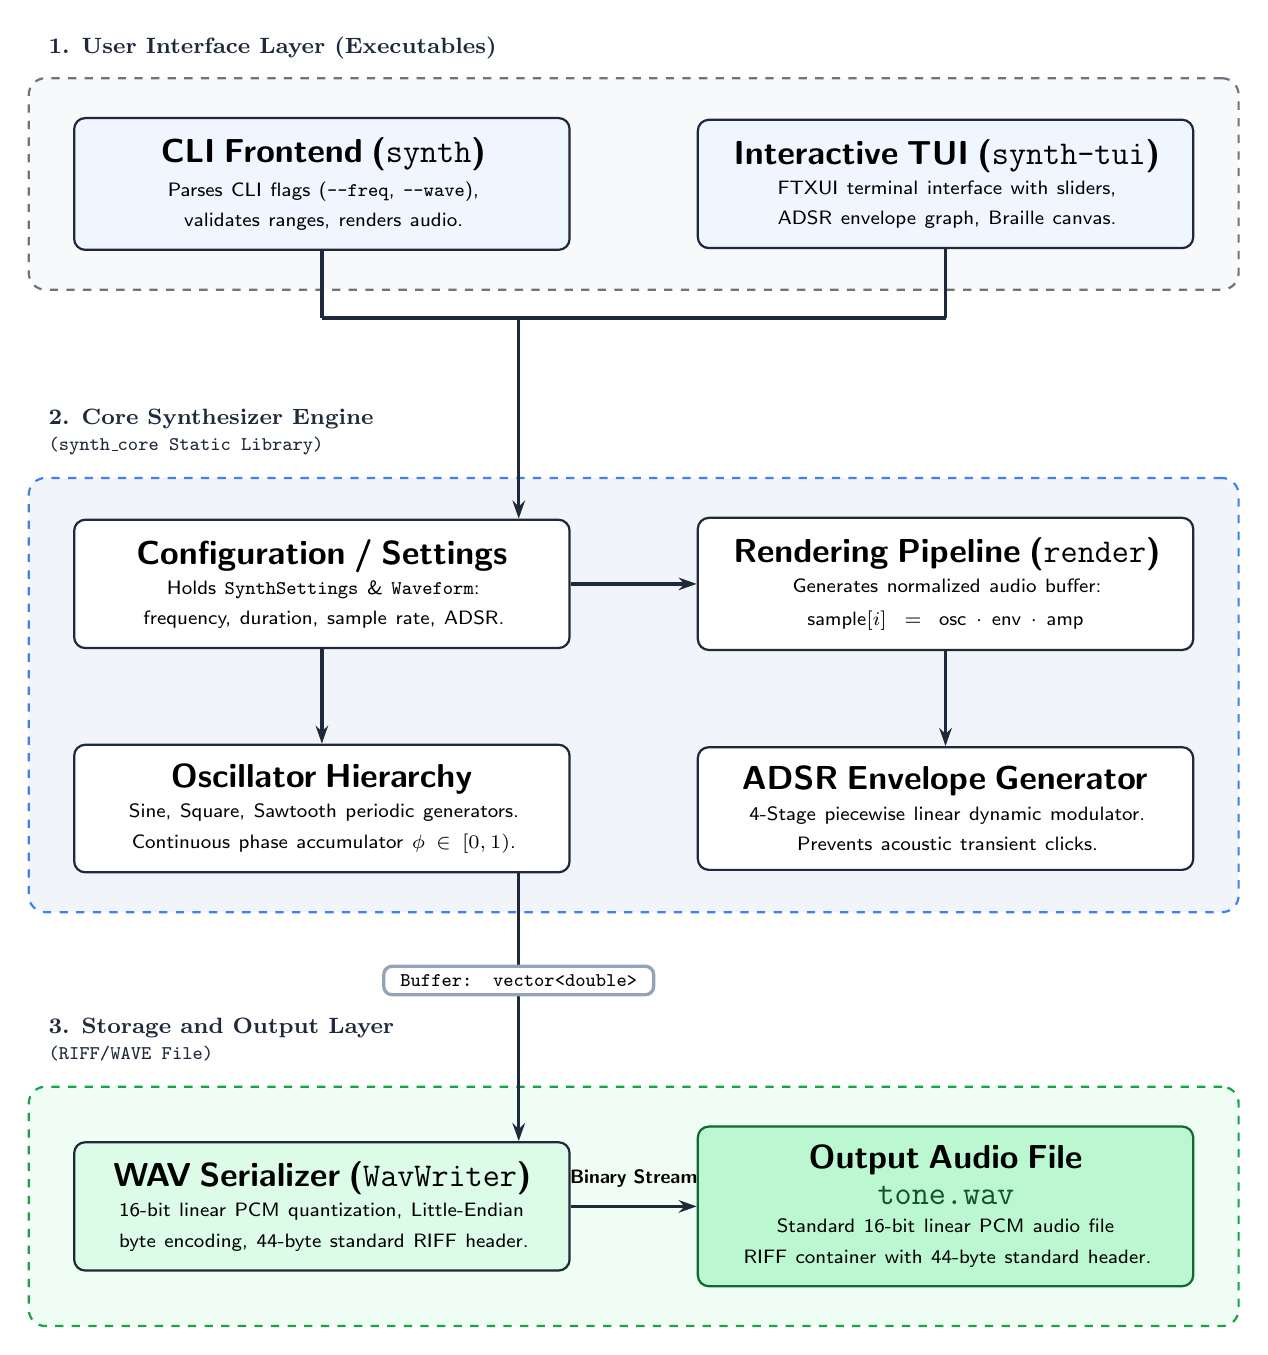
\begin{tikzpicture}[
    font=\small\sffamily,
    box/.style={
        draw=darkborder,
        thick,
        fill=white,
        rounded corners=4pt,
        align=center,
        inner sep=7pt
    },
    flowArrow/.style={
        -{Stealth[length=6.5pt, width=4.5pt]},
        very thick,
        draw=darkborder
    }
]

    % =========================================================================
    % LAYER 1: USER INTERFACE LAYER
    % =========================================================================
    \node[box, fill=uiboxbg, text width=5.8cm] (cli) at (0, 0) {
        \textbf{\large CLI Frontend (\texttt{synth})}\\[3pt]
        \scriptsize Parses CLI flags (\texttt{--freq}, \texttt{--wave}),\\validates ranges, renders audio.
    };

    \node[box, fill=uiboxbg, text width=5.8cm, right=1.6cm of cli] (tui) {
        \textbf{\large Interactive TUI (\texttt{synth-tui})}\\[3pt]
        \scriptsize FTXUI terminal interface with sliders,\\ADSR envelope graph, Braille canvas.
    };

    \begin{scope}[on background layer]
        \node[fill=layer1bg, draw=layer1border, dashed, thick, rounded corners=6pt,
              fit=(cli) (tui), inner xsep=16pt, inner ysep=14pt] (layer1) {};
    \end{scope}

    \node[anchor=south west, font=\bfseries\footnotesize, text=darkborder] 
          at ([xshift=4pt, yshift=3pt]layer1.north west) {1. User Interface Layer (Executables)};

    % =========================================================================
    % LAYER 2: CORE SYNTHESIZER ENGINE
    % =========================================================================
    \node[box, fill=white, text width=5.8cm, below=3.4cm of cli] (settings) {
        \textbf{\large Configuration / Settings}\\[3pt]
        \scriptsize Holds \texttt{SynthSettings} \& \texttt{Waveform}:\\frequency, duration, sample rate, ADSR.
    };

    \node[box, fill=white, text width=5.8cm, right=1.6cm of settings] (pipeline) {
        \textbf{\large Rendering Pipeline (\texttt{render})}\\[3pt]
        \scriptsize Generates normalized audio buffer:\\[1pt]
        $\text{sample}[i] = \text{osc} \cdot \text{env} \cdot \text{amp}$
    };

    \node[box, fill=white, text width=5.8cm, below=1.2cm of settings] (oscSub) {
        \textbf{\large Oscillator Hierarchy}\\[3pt]
        \scriptsize Sine, Square, Sawtooth periodic generators.\\Continuous phase accumulator $\phi \in [0, 1)$.
    };

    \node[box, fill=white, text width=5.8cm, right=1.6cm of oscSub] (envSub) {
        \textbf{\large ADSR Envelope Generator}\\[3pt]
        \scriptsize 4-Stage piecewise linear dynamic modulator.\\Prevents acoustic transient clicks.
    };

    \begin{scope}[on background layer]
        \node[fill=layer2bg, draw=layer2border, dashed, thick, rounded corners=6pt,
              fit=(settings) (pipeline) (oscSub) (envSub), inner xsep=16pt, inner ysep=14pt] (layer2) {};
    \end{scope}

    \node[anchor=south west, font=\bfseries\footnotesize, text=darkborder] 
          at ([xshift=4pt, yshift=3pt]layer2.north west) {\begin{tabular}{@{}l@{}}\textbf{2. Core Synthesizer Engine}\\\scriptsize\texttt{(synth\_core Static Library)}\end{tabular}};

    % =========================================================================
    % LAYER 3: STORAGE & FILE OUTPUT
    % =========================================================================
    \node[box, fill=writerbg, text width=5.8cm, below=3.4cm of oscSub] (wavWriter) {
        \textbf{\large WAV Serializer (\texttt{WavWriter})}\\[3pt]
        \scriptsize 16-bit linear PCM quantization, Little-Endian\\byte encoding, 44-byte standard RIFF header.
    };

    \node[box, fill=filebg, draw=fileborder, text width=5.8cm, right=1.6cm of wavWriter] (wavFile) {
        \textbf{\large Output Audio File}\\[2pt]
        \textbf{\large\textcolor{filetext}{\texttt{tone.wav}}}\\[2pt]
        \scriptsize Standard 16-bit linear PCM audio file\\RIFF container with 44-byte standard header.
    };

    \begin{scope}[on background layer]
        \node[fill=layer3bg, draw=layer3border, dashed, thick, rounded corners=6pt,
              fit=(wavWriter) (wavFile), inner xsep=16pt, inner ysep=14pt] (layer3) {};
    \end{scope}

    \node[anchor=south west, font=\bfseries\footnotesize, text=darkborder] 
          at ([xshift=4pt, yshift=3pt]layer3.north west) {\begin{tabular}{@{}l@{}}\textbf{3. Storage and Output Layer}\\\scriptsize\texttt{(RIFF/WAVE File)}\end{tabular}};

    % =========================================================================
    % DATAFLOW ARROWS & BUS
    % =========================================================================
    % Dynamic UI Bus Calculation: using pos=0.25 keeps the horizontal line securely above the text[cite: 15]
    \path (cli.south) -- (settings.north) coordinate[pos=0.25] (midUI);
    
    \draw[very thick, draw=darkborder] (cli.south) -- (cli.south |- midUI);
    \draw[very thick, draw=darkborder] (tui.south) -- (tui.south |- midUI);
    \draw[very thick, draw=darkborder] (cli.south |- midUI) -- (tui.south |- midUI);
    
    % Downward arrow shifted securely right (x=2.5cm) to clear the Layer 2 text box perfectly[cite: 15]
    \draw[flowArrow] ([xshift=2.5cm]settings.north |- midUI) -- ([xshift=2.5cm]settings.north);

    % Internal Layer 2 Dataflow
    \draw[flowArrow] (settings.east) -- (pipeline.west);
    \draw[flowArrow] (settings.south) -- (oscSub.north);
    \draw[flowArrow] (pipeline.south) -- (envSub.north);

    % Downward arrow to Layer 3 shifted identically to clear the Layer 3 text box perfectly[cite: 15]
    \draw[flowArrow] ([xshift=2.5cm]oscSub.south) -- 
        node[pos=0.4, fill=white, draw=badgeborder, rounded corners=3pt, inner xsep=6pt, inner ysep=3pt, font=\scriptsize\ttfamily] {Buffer: \texttt{vector<double>}} 
        ([xshift=2.5cm]wavWriter.north);

    % Horizontal write to output file
    \draw[flowArrow] (wavWriter.east) -- node[midway, above=3pt, font=\scriptsize\bfseries\sffamily] {Binary Stream} (wavFile.west);

\end{tikzpicture}
}
\caption{Three-tier decoupled architectural diagram of the Audio-WAV-Synthesizer.}
\label{fig:sys_arch}
\end{figure}

% FloatBarrier guarantees Figure 24.1 appears strictly BEFORE Figure 24.2
\FloatBarrier

% ---------------------------------------------------------------------
% 24.4.1 UML CLASS DIAGRAM
% ---------------------------------------------------------------------
\subsection{UML Class Diagram}
Figure~\ref{fig:uml_class} formally specifies the static structural model of the system, precisely matching the canonical object model. The abstract class \texttt{Oscillator} defines the virtual interface \texttt{nextSample() = 0} and encapsulates normalized phase state $\phi$. Concrete subclasses (\texttt{SineOscillator}, \texttt{SquareOscillator}, \texttt{SawtoothOscillator}) inherit phase tracking while providing distinct waveform evaluation logic.

\begin{figure}[htbp]
\centering
\resizebox{0.95\textwidth}{!}{%
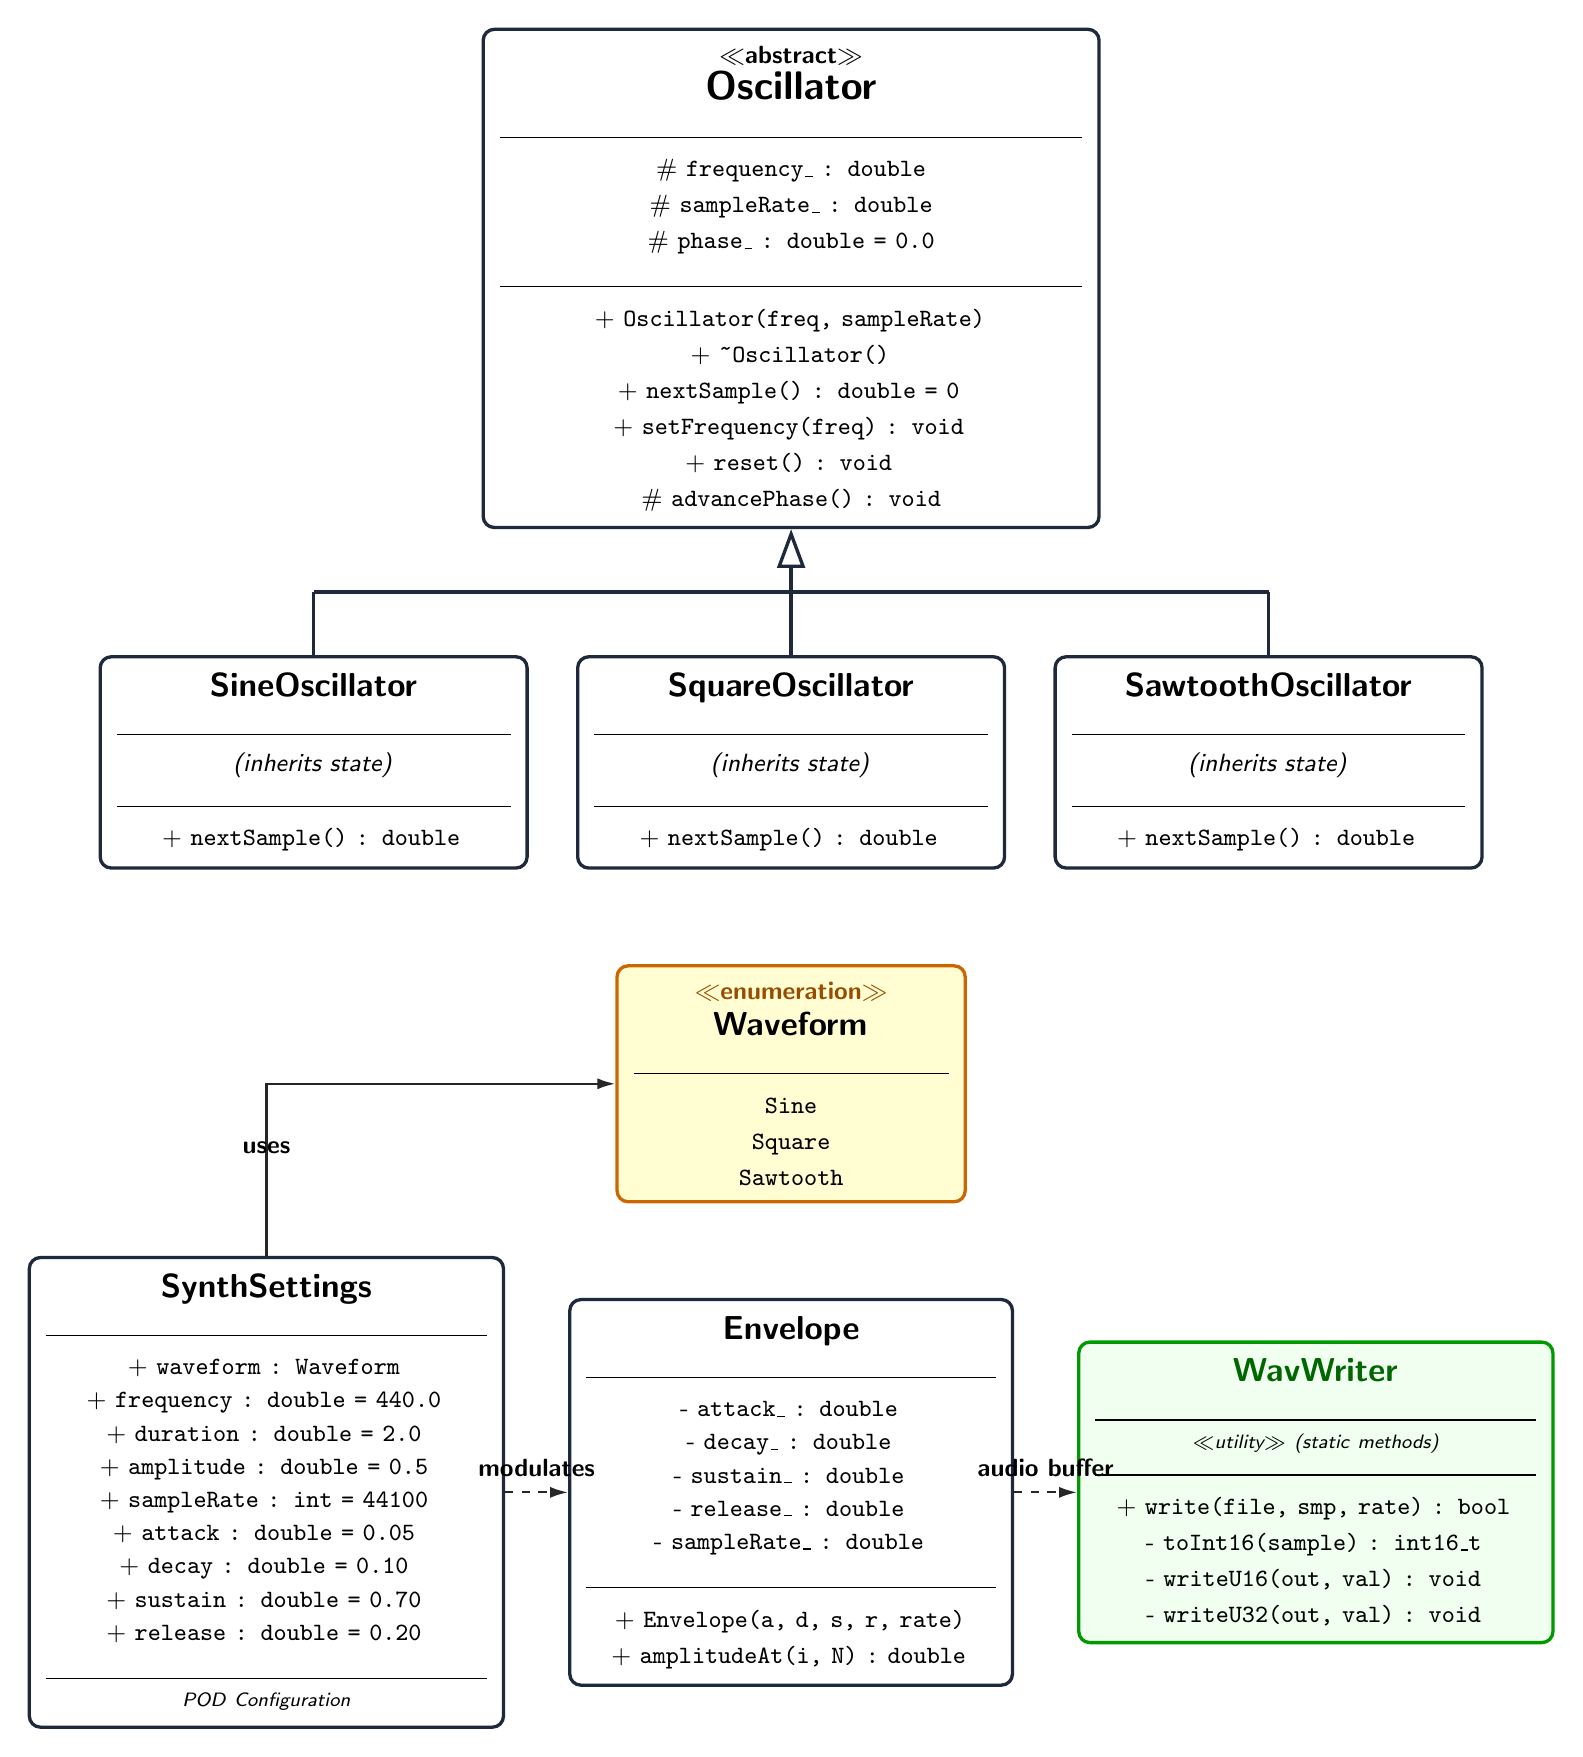
\begin{tikzpicture}[
    font=\small\sffamily,
    umlClass/.style={
        draw=darkborder,
        very thick,
        fill=white,
        rounded corners=4pt,
        inner sep=6pt,
        align=left
    },
    umlAbstract/.style={
        umlClass,
        fill=white
    },
    umlEnum/.style={
        umlClass,
        fill=yellow!18,
        draw=orange!80!black
    },
    umlWriter/.style={
        umlClass,
        fill=green!6,
        draw=green!60!black
    },
    depend/.style={
        -{Latex[length=6.5pt, width=4pt]},
        dashed,
        thick,
        draw=black!85
    },
    assoc/.style={
        -{Latex[length=6.5pt, width=4pt]},
        thick,
        draw=black!85
    }
]

    % =========================================================================
    % TIER 1: Abstract Base Class (Oscillator)
    % =========================================================================
    \node[umlAbstract, text width=7.4cm] (oscillator) at (0, 0) {
        \centering $\ll$\textbf{abstract}$\gg$\\[2pt]
        \centering\textbf{\Large Oscillator}\\[3pt]
        \rule{\linewidth}{0.5pt}\\[3pt]
        \small
        \# \texttt{frequency\_ : double}\\[2pt]
        \# \texttt{sampleRate\_ : double}\\[2pt]
        \# \texttt{phase\_ : double = 0.0}\\[3pt]
        \rule{\linewidth}{0.5pt}\\[3pt]
        \small
        + \texttt{Oscillator(freq, sampleRate)}\\[2pt]
        + \texttt{\textasciitilde Oscillator()}\\[2pt]
        + \texttt{nextSample() : double = 0}\\[2pt]
        + \texttt{setFrequency(freq) : void}\\[2pt]
        + \texttt{reset() : void}\\[2pt]
        \# \texttt{advancePhase() : void}\\[1pt]
    };

    % =========================================================================
    % TIER 2: Derived Oscillators
    % =========================================================================
    \node[umlClass, text width=5.0cm, below=1.6cm of oscillator] (squareOsc) {
        \centering\textbf{\large SquareOscillator}\\[3pt]
        \rule{\linewidth}{0.5pt}\\[2pt]
        \centering\small\textit{(inherits state)}\\[2pt]
        \rule{\linewidth}{0.5pt}\\[3pt]
        \small + \texttt{nextSample() : double}\\[1pt]
    };

    \node[umlClass, text width=5.0cm, left=0.6cm of squareOsc] (sineOsc) {
        \centering\textbf{\large SineOscillator}\\[3pt]
        \rule{\linewidth}{0.5pt}\\[2pt]
        \centering\small\textit{(inherits state)}\\[2pt]
        \rule{\linewidth}{0.5pt}\\[3pt]
        \small + \texttt{nextSample() : double}\\[1pt]
    };

    \node[umlClass, text width=5.0cm, right=0.6cm of squareOsc] (sawOsc) {
        \centering\textbf{\large SawtoothOscillator}\\[3pt]
        \rule{\linewidth}{0.5pt}\\[2pt]
        \centering\small\textit{(inherits state)}\\[2pt]
        \rule{\linewidth}{0.5pt}\\[3pt]
        \small + \texttt{nextSample() : double}\\[1pt]
    };

    % =========================================================================
    % INHERITANCE BUS BAR & STEMS
    % =========================================================================
    % Compute a dynamic coordinate halfway between Oscillator bottom and SquareOscillator top
    \path (oscillator.south) -- (squareOsc.north) coordinate[midway] (bus);

    % Main upward hollow triangle pointer to the base class
    \draw[very thick, draw=darkborder, -{Triangle[open, length=14pt, width=10pt]}] (bus) -- (oscillator.south);

    % Horizontal distribution bus bar
    \draw[very thick, draw=darkborder] (sineOsc.north |- bus) -- (sawOsc.north |- bus);

    % Vertical drops to the three derived classes
    \draw[very thick, draw=darkborder] (sineOsc.north |- bus) -- (sineOsc.north);
    \draw[very thick, draw=darkborder] (squareOsc.north |- bus) -- (squareOsc.north);
    \draw[very thick, draw=darkborder] (sawOsc.north |- bus) -- (sawOsc.north);

    % =========================================================================
    % TIER 3: Waveform Enumeration
    % =========================================================================
    \node[umlEnum, text width=4.0cm, below=1.2cm of squareOsc] (waveformEnum) {
        \centering\textcolor{orange!60!black}{\textbf{$\ll$enumeration$\gg$}}\\[2pt]
        \centering\textbf{\large Waveform}\\[3pt]
        \rule{\linewidth}{0.5pt}\\[3pt]
        \centering\small
        \texttt{Sine}\\[2pt]
        \texttt{Square}\\[2pt]
        \texttt{Sawtooth}\\[1pt]
    };

    % =========================================================================
    % TIER 4: Bottom Row (Envelope, SynthSettings, WavWriter)
    % =========================================================================
    \node[umlClass, text width=5.2cm, below=1.2cm of waveformEnum] (envelope) {
        \centering\textbf{\large Envelope}\\[3pt]
        \rule{\linewidth}{0.5pt}\\[3pt]
        \small
        - \texttt{attack\_ : double}\\[1pt]
        - \texttt{decay\_ : double}\\[1pt]
        - \texttt{sustain\_ : double}\\[1pt]
        - \texttt{release\_ : double}\\[1pt]
        - \texttt{sampleRate\_ : double}\\[3pt]
        \rule{\linewidth}{0.5pt}\\[3pt]
        \small
        + \texttt{Envelope(a, d, s, r, rate)}\\[2pt]
        + \texttt{amplitudeAt(i, N) : double}\\[2pt]
    };

    \node[umlClass, text width=5.6cm, left=0.8cm of envelope] (settings) {
        \centering\textbf{\large SynthSettings}\\[3pt]
        \rule{\linewidth}{0.5pt}\\[3pt]
        \small
        + \texttt{waveform : Waveform}\\[1pt]
        + \texttt{frequency : double = 440.0}\\[1pt]
        + \texttt{duration : double = 2.0}\\[1pt]
        + \texttt{amplitude : double = 0.5}\\[1pt]
        + \texttt{sampleRate : int = 44100}\\[1pt]
        + \texttt{attack : double = 0.05}\\[1pt]
        + \texttt{decay : double = 0.10}\\[1pt]
        + \texttt{sustain : double = 0.70}\\[1pt]
        + \texttt{release : double = 0.20}\\[3pt]
        \rule{\linewidth}{0.5pt}\\[2pt]
        \centering\scriptsize\textit{POD Configuration}\\[1pt]
    };

    \node[umlWriter, text width=5.6cm, right=0.8cm of envelope] (wavWriter) {
        \centering\textbf{\large\textcolor{green!40!black}{WavWriter}}\\[3pt]
        \rule{\linewidth}{0.5pt}\\[2pt]
        \centering\scriptsize\textit{$\ll$utility$\gg$ (static methods)}\\[2pt]
        \rule{\linewidth}{0.5pt}\\[3pt]
        \small
        + \texttt{write(file, smp, rate) : bool}\\[2pt]
        - \texttt{toInt16(sample) : int16\_t}\\[2pt]
        - \texttt{writeU16(out, val) : void}\\[2pt]
        - \texttt{writeU32(out, val) : void}\\[2pt]
    };

    % =========================================================================
    % ARROWS & ASSOCIATIONS
    % =========================================================================
    % SynthSettings -> Waveform: Orthogonal route going UP and right into the face
    \draw[assoc] (settings.north) |- 
        node[near start, above=2pt, font=\small\bfseries\sffamily] {uses} (waveformEnum.west);

    % SynthSettings -> Envelope: Dashed horizontal connection
    \draw[depend] (settings.east) -- 
        node[midway, above=2pt, font=\small\bfseries\sffamily] {modulates} (envelope.west);

    % Envelope -> WavWriter: Dashed horizontal connection
    \draw[depend] (envelope.east) -- 
        node[midway, above=2pt, font=\small\bfseries\sffamily] {audio buffer} (wavWriter.west);

\end{tikzpicture}
}
\caption{UML Class Diagram: Depicts the polymorphic base interface \texttt{Oscillator}, derived concrete waveforms, configuration encapsulation via \texttt{SynthSettings}, temporal envelope shaping, and static binary serialization.}
\label{fig:uml_class}
\end{figure}

\FloatBarrier
    
% =====================================================================
% 24.5 LOW-LEVEL BINARY RIFF/WAVE SERIALIZATION
% =====================================================================
\section{Low-Level Binary RIFF/WAVE Serialization}
Listing~\ref{lst:wavwriter_cpp} documents the low-level binary serialization implementation. The static method quantizes floating-point samples to 16-bit signed integers ($[-32768, 32767]$) and formats the canonical 44-byte RIFF/WAVE header directly into an unbuffered binary \texttt{std::ofstream}.

\begin{lstlisting}[language=C++, caption={Raw Binary RIFF/WAVE File Serializer (\texttt{src/WavWriter.cpp})}, label={lst:wavwriter_cpp}]
#include "WavWriter.h"
#include <algorithm>
#include <cmath>
#include <fstream>

std::int16_t WavWriter::toInt16(double sample) {
    sample = std::clamp(sample, -1.0, 1.0);
    return static_cast<std::int16_t>(std::lround(sample * 32767.0));
}

void WavWriter::writeU16(std::ostream& out, std::uint16_t value) {
    const char bytes[2] = {
        static_cast<char>(value & 0xFF),
        static_cast<char>((value >> 8) & 0xFF)
    };
    out.write(bytes, 2);
}

void WavWriter::writeU32(std::ostream& out, std::uint32_t value) {
    const char bytes[4] = {
        static_cast<char>(value & 0xFF),
        static_cast<char>((value >> 8) & 0xFF),
        static_cast<char>((value >> 16) & 0xFF),
        static_cast<char>((value >> 24) & 0xFF)
    };
    out.write(bytes, 4);
}

bool WavWriter::write(const std::string& filename,
                      const std::vector<double>& samples,
                      std::uint32_t sampleRate,
                      std::uint16_t channels) {
    std::ofstream file(filename, std::ios::binary);
    if (!file) return false;

    const std::uint16_t bitsPerSample = 16;
    const std::uint16_t blockAlign = channels * bitsPerSample / 8;
    const std::uint32_t byteRate = sampleRate * blockAlign;
    const std::uint32_t dataSize = static_cast<std::uint32_t>(samples.size() * 2);
    const std::uint32_t chunkSize = 36 + dataSize;

    // 1. RIFF Container Header
    file.write("RIFF", 4);
    writeU32(file, chunkSize);
    file.write("WAVE", 4);

    // 2. Format Chunk ("fmt ")
    file.write("fmt ", 4);
    writeU32(file, 16);               // Subchunk1Size (16 for PCM)
    writeU16(file, 1);                // AudioFormat (1 = PCM uncompressed)
    writeU16(file, channels);         // NumChannels (1 = Mono)
    writeU32(file, sampleRate);       // SampleRate (e.g. 44100 Hz)
    writeU32(file, byteRate);         // ByteRate
    writeU16(file, blockAlign);       // BlockAlign
    writeU16(file, bitsPerSample);    // BitsPerSample (16 bits)

    // 3. Data Chunk ("data")
    file.write("data", 4);
    writeU32(file, dataSize);

    // 4. Quantized PCM Little-Endian Sample Streaming
    std::vector<char> buffer(samples.size() * 2);
    for (std::size_t i = 0; i < samples.size(); ++i) {
        const std::uint16_t v = static_cast<std::uint16_t>(toInt16(samples[i]));
        buffer[2 * i]     = static_cast<char>(v & 0xFF);
        buffer[2 * i + 1] = static_cast<char>((v >> 8) & 0xFF);
    }
    file.write(buffer.data(), static_cast<std::streamsize>(buffer.size()));

    file.close();
    return !file.fail();
}
\end{lstlisting}

Table~\ref{tab:riff_header} summarizes the exact 44-byte structure assembled by \texttt{WavWriter}.

\begin{table}[htbp]
\centering
\caption{Canonical 44-Byte Microsoft RIFF/WAVE Header Specification}
\label{tab:riff_header}
\footnotesize
\begin{tabular}{@{}llllp{6.8cm}@{}}
\toprule
\textbf{Offset} & \textbf{Field Name} & \textbf{Size} & \textbf{Endianness} & \textbf{Semantic Value / Role} \\ \midrule
0 & \texttt{ChunkID} & 4 Bytes & Big & \texttt{"RIFF"} ASCII signature \\
4 & \texttt{ChunkSize} & 4 Bytes & Little & $36 + \text{DataSize}$ (Total file size $- 8$) \\
8 & \texttt{Format} & 4 Bytes & Big & \texttt{"WAVE"} container type \\
12 & \texttt{Subchunk1ID} & 4 Bytes & Big & \texttt{"fmt "} format chunk marker \\
16 & \texttt{Subchunk1Size} & 4 Bytes & Little & 16 for uncompressed Linear PCM \\
20 & \texttt{AudioFormat} & 2 Bytes & Little & 1 specifies Linear PCM \\
22 & \texttt{NumChannels} & 2 Bytes & Little & 1 for Mono, 2 for Stereo \\
24 & \texttt{SampleRate} & 4 Bytes & Little & Sampling frequency $f_s$ in Hz (e.g., 44100) \\
28 & \texttt{ByteRate} & 4 Bytes & Little & $\text{SampleRate} \times \text{Channels} \times \frac{\text{Bits}}{8}$ \\
32 & \texttt{BlockAlign} & 2 Bytes & Little & $\text{Channels} \times \frac{\text{Bits}}{8}$ (2 for 16-bit mono) \\
34 & \texttt{BitsPerSample} & 2 Bytes & Little & 16 bits quantization depth \\
36 & \texttt{Subchunk2ID} & 4 Bytes & Big & \texttt{"data"} payload identifier \\
40 & \texttt{Subchunk2Size} & 4 Bytes & Little & $N_{\text{samples}} \times \text{Channels} \times \frac{\text{Bits}}{8}$ \\
\bottomrule
\end{tabular}
\end{table}

\FloatBarrier

% =====================================================================
% 24.6 CONCLUSION 
% =====================================================================
\section{Conclusion}
The Audio Synthesizer and WAV Generator project demonstrates the design of a decoupled, performant, and extensible software synthesizer implemented in modern C++17. By applying foundational Object-Oriented principles—including pure virtual polymorphic dispatch, dynamic inheritance hierarchies, strict state encapsulation, and modular architectural separation—the application successfully bridges mathematical acoustics with systems-level binary file serialization.

Key milestones accomplished include:
\begin{itemize}
    \item Developed an extensible abstract oscillator base hierarchy enabling straightforward addition of future waveform types.
    \item Eliminated audio click transients through a 4-stage piecewise linear ADSR envelope generator.
    \item Implemented direct low-level 16-bit little-endian RIFF/WAVE binary stream writing without external multimedia runtime dependencies.
    \item Provided dual frontends: a command-line interface for automated batch processing and an interactive terminal GUI powered by FTXUI.
\end{itemize}

\end{document}
